\section{Methodology}
For our research we adopted the SLR method, so that we can analyze the relevant literature. SLRs are designed to provide an overview of the existing literature on a specific topic area ~\cite{frizzo-barker_blockchain_2020}. They are commonly used in the medical field and have been increasingly adopted by scientists as a tool in emerging fields.

\subsection{Research Questions}
Firstly, we define a set of research questions which help to narrow the wide topic of "Process and Blockchain". The following research questions were used as a guide to further examine the role blockchain can play in BPM.
\begin{enumerate}
    \item \textbf{How can BPM take advantage of blockchain technologies?} 
    
    %This question was laid out to identify the potential benefits and opportunities that blockchain technologies can bring to the field of business process management. By investigating the ways in which blockchain can optimize and streamline processes, this question can provide valuable insights into how companies can improve their operations and gain a competitive advantage.
    
    \item \textbf{What are the top challenges and risks associated with integrating blockchain in BPM?}
    
    %With this question we highlight the potential drawbacks and obstacles that companies may encounter when incorporating blockchain technologies into their operations. By identifying these challenges and risks, this question can provide guidance on how to mitigate them and ensure the successful implementation of blockchain in business process management.
    
    \item \textbf{Which applications of blockchain in BPM have been proposed and how are they evaluated?}

    %Providing an overview of the different ways in which blockchain technologies have been applied in the field of business process management is beneficial in deciding where future research and development efforts should be directed. By identifying the various proposals for blockchain-based solutions and evaluating their effectiveness, this question can give an insight into the state of the art of blockchain in BPM and provide a basis for future research.
\end{enumerate}

\subsection{Search Strategy}
Next, it is important to use a comprehensive search strategy in order to identify relevant studies. In this case, the databases chosen are IEEExplore, ScienceDirect, Springer Link and ACM Digital Library. These databases are widely used in academic research and are likely to contain relevant and high quality studies on the topic of blockchain in BPM. 
\setlength{\tabcolsep}{3em}
\begin{table}[]
    \centering
    \caption{Search keywords}
    \begin{tabular}{l r}
        \hline
        A & B \\
        \hline\hline
        Blockchain & Business Process\\
        Distributed Ledger &  Business Process Management\\
        DLT & BPM \\
        Smart contract &  \\
        Ethereum & \\
        \hline
    \end{tabular}
    \label{tab:keywords}
\end{table}

A combination of the search terms seen in Table \ref{tab:keywords} above were used to create the search string. Most databases we searched allowed using the logical operators (such as AND, OR, NOT) to combine all the terms in one search string and therefore avoid duplications.  The final search string was "(blockchain OR distributed ledger OR DLT OR smart contract OR ethereum) AND (business process OR business process management OR BPM)". Using the search string, we conducted a search in each of the selected databases. The search was conducted on November 2022 by using the following fields: title, abstract, and keywords. We already limited our search to English studies published between 2020 and 2022, according to our study selection criteria further explained in \ref{ssec:study-selection}. At this stage, the search resulted in 1659 documents being identified.

\subsection{Study Selection} \label{ssec:study-selection}
In the third phase, we use different selection criteria to define the parameters of the studies that will be included in the SLR. Applying these criteria makes sure that we identified studies with high relevance and quality. Studies were included if they fulfilled at least one of the following inclusion criteria:
\begin{enumerate}
    \item Studies that examine the use of blockchain in the BPM lifecycle.
    \item Studies that present a new solution to integrating blockchain in BPM.
    \item Studies that extends a blockchain-based solution for BPM.
\end{enumerate}

%To ensure a focus on high-quality work, some articles that were deemed irrelevant, low-quality, or of low importance were removed. 
\noindent The following were the exclusion criteria used to discard irrelevant studies.
\begin{enumerate}
    \item Studies not written in English.
    \item Studies not published between 2020 and 2022.
    \item Studies with no reviewers.
    \item Non primary studies.
    \item Studies which handle a specific application area (such as supply chain management) and are not intended for BPs and BPM in general.
\end{enumerate}
To implement the criteria, we first filtered the results by reading the title which reduced the documents from 1659 to 71 potential papers. Then, by reading the abstract and skimming through the key contents of the papers we reduced this number further down to 11. Searching the citations yielded two different papers bringing the total of selected studies to 13.

\begin{figure}
    \centering
    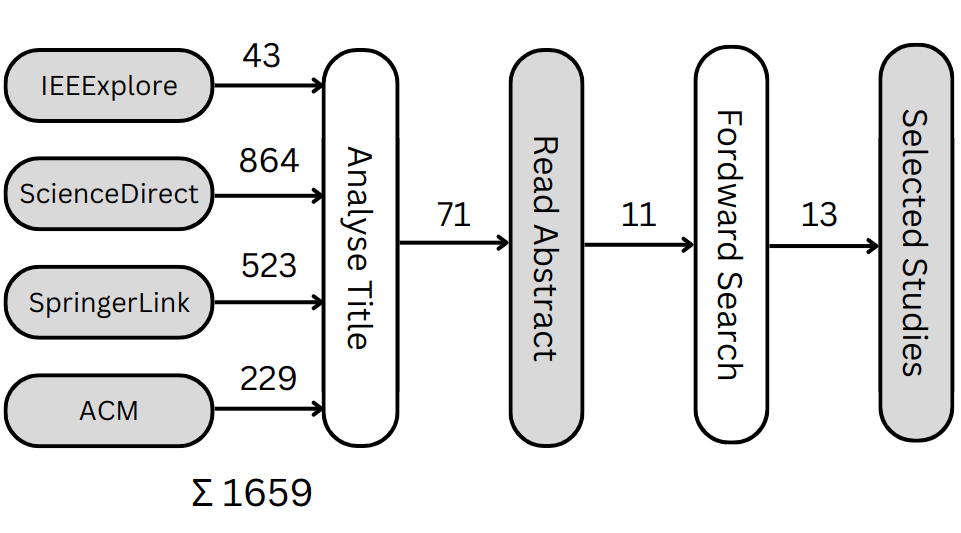
\includegraphics[width=\textwidth]{search-final.png}
    \caption{Search timeline}
    \label{fig:search}
\end{figure}